\documentclass{report}
\usepackage[margin=1in, paperwidth=8.5in, paperheight=11in]{geometry}
%Math packages%
\usepackage{amsmath}
\usepackage{amsthm}
%Spacing%
\usepackage{setspace}
\onehalfspacing
%Lecture number%
\newcommand{\lectureNum}{13}
%Variables - Date and Course%
\newcommand{\curDate}{February 14, 2017}
\newcommand{\course}{CS 241}
\newcommand{\instructor}{Kevin Lanctot}
%Defining the example tag%
%\theoremstyle{definition}%
\newtheorem{ex}{Example}[section]
%Setting counter given the lecture number%
\setcounter{chapter}{\lectureNum{}}
%Package to insert code%
\usepackage{listings}
\usepackage{courier}
\usepackage{xcolor}
\lstset { %
    tabsize=2,
    breaklines=true,
    language=C++,
    backgroundcolor=\color{blue!8}, % set backgroundcolor
    basicstyle=\footnotesize\ttfamily,% basic font setting
}
%Package for images%
\usepackage{graphicx}

\begin{document}
%Note title%
\begin{center}
\begin{Large}
\textsc{\course{} | Lecture \lectureNum{}}
\end{Large}
\end{center} 
\noindent \textit{Bartosz Antczak} \hfill
\textit{Instructor: \instructor{}} \hfill
\textit{\curDate{}}
\rule{\textwidth}{0.4pt}
% Actual Notes%
\subsubsection{Recall: Context-Free Grammar}
Since DFA's, NFA's, and regular expressions are finite, they won't suffice in reading the syntax. We'll need something more powerful, and from that stems \textbf{context-free grammar}, which is an approach to interpreting a sequence of tokens and determining if the syntax of a program is correct.
\section{Examples of Context-free Grammar}
Context-free Grammar (CFG) involves a set of rules that we can use to manipulate words found in a language.

\subsection{Example 1}
\begin{figure}[ht]
\begin{center}
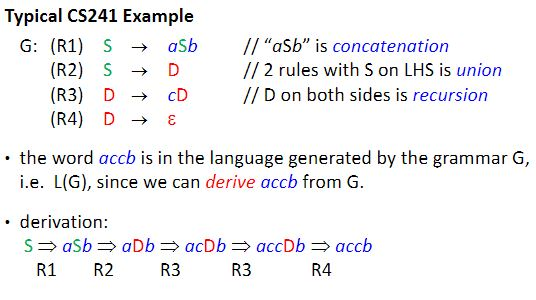
\includegraphics[scale=0.8]{cfg1.jpg}
\end{center}
\caption{We can derive the word ``accb" using this particular CFG. This means that ``accb" is a valid word in the language. Courtesy of Prof. Lanctot's slides.} 
\end{figure}
\subsection{Example 2}
Consider the language $\Sigma = \{a,b\}$ whose language consists of words that start with one `a', followed by an arbitrary amount of `b's (i.e., $\{a, ab, abb, abbb, \cdots\}$). The rules of the CFG that reads this language are:
\begin{itemize}
\item \textbf{(R1)}: $S \rightarrow aB$
\item \textbf{(R2)}: $B \rightarrow bB$
\item \textbf{(R3)}: $B \rightarrow \varepsilon$
\end{itemize}
Say we want to derive $abb$, we would do the following:
$$S \rightarrow_{(R1)} aB \rightarrow_{(R2)} abB \rightarrow_{(R2)} abbB \rightarrow_{(R3)} abb$$
\subsection{Example 3}
Let's create a CFG that access accepts words with balanced parentheses. For example, valid words are
$$\varepsilon, \, (), \, (()),\, ()(),\, (()()), \cdots$$
The rules in the grammar are:
\begin{itemize}
\item \textbf{(R1)}: $S \rightarrow (S)$
\item \textbf{(R2)}: $S \rightarrow S \,\, S$
\item \textbf{(R3)}: $S \rightarrow \varepsilon$
\end{itemize}
From these, let's derive some words:
\begin{enumerate}
\item Derive $(())$: 
$$S \rightarrow_{(R1)} (S) \rightarrow_{(R1)} ((S)) \rightarrow_{(R3)} (())$$
\item Derive $(()())$:
$$S \rightarrow_{(R1)} (S) \rightarrow_{(R2)} (S S) \rightarrow_{(R1)} ((S) S ) \rightarrow_{(R3)} (() S) \rightarrow_{(R1)} (() (S)) \rightarrow_{(R3)} (()())$$
\end{enumerate}
\subsection{Example 4}
For $\Sigma = \{a,b\}$, a CFG that contains an even number of a's:
\begin{itemize}
\item \textbf{(R1)}: $S \rightarrow bS$
\item \textbf{(R2)}: $S \rightarrow Sb$
\item \textbf{(R3)}: $S \rightarrow aSa$ (a's are generated in pairs, which grantees that we have an even number)
\item \textbf{(R4)}: $S \rightarrow \varepsilon$
\end{itemize}

\subsection{Example 5}
Binary Expressions
\begin{figure}[ht]
\begin{center}
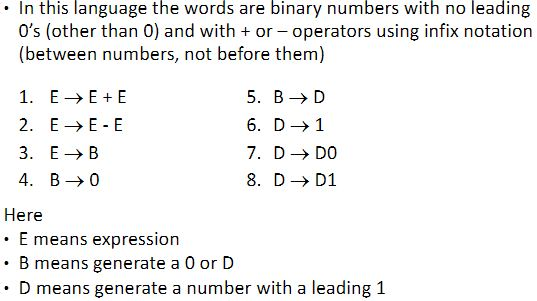
\includegraphics[scale=0.5]{cfg2.jpg}
\end{center}
\caption{Courtesy of Prof. Lanctot's slides.}
\end{figure}
\section{Parse Trees}
Also called a \textit{derivation tree}. It visualizes an entire derivation at once. The tree is structured such that:
\begin{itemize}
\item The \textbf{internal nodes} are the non-terminals (e.g., E, B, D)
\item The \textbf{root} of the tree is the start symbol (e.g., E)
\item The \textbf{children} of a node are given by derivation rules
\item The \textbf{leaf nodes} are the terminals and show their value (e.g., $1, 0, + 1$)
\end{itemize}
\subsubsection{Ambiguous Grammar}
Because grammar can be ambiguous, we can have multiple parse trees for the same expression.\\
The way we'll be processing order in a parse tree is with a \textbf{post-order} with a \textbf{depth first} traversal.
\subsubsection{Unambiguous Grammar}
To make CFG unambiguous, we must change our rules:
\begin{figure}[ht]
\begin{center}
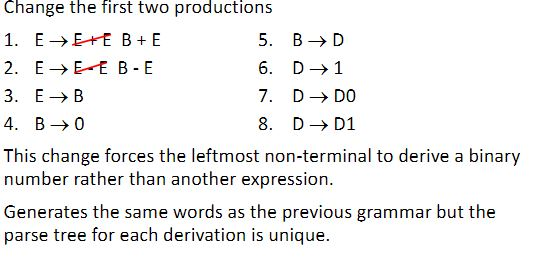
\includegraphics[scale=0.7]{cfg3.jpg}
\end{center}
\caption{Courtesy of Prof. Lanctot's slides.}
\end{figure}
%END%
\end{document}